%%%%%%%%%%%%%%%%%%%%%%%%%%%%%%%%%%%%%%%%%%%%%%%%%%%%%%%%%%%%%%%%%
% Contents : The budgetary lines chapter
% $Id : grisbi-manuel-budgetlines.tex, v 0.4 2002/10/27 Daniel Cartron
% $Id : grisbi-manuel-budgetlines.tex, v 0.5.0 2004/06/01 Loic Breilloux
% some of its content was in tips chapter  : 
% $Id : grisbi-manuel-tips.tex, v 0.4 2002/10/27 Daniel Cartron
% $Id : grisbi-manuel-budgetlines.tex, v 0.6.0 2011/11/17 Jean-Luc Duflot
% some of its content was in tips chapter  :
% $Id : grisbi-manuel-tips.tex, v 0.5.0 2004/06/01 Loic Breilloux
% $Id : grisbi-manuel-budgetlines.tex, v 0.8.9 2012/04/27 Jean-Luc Duflot
% $Id : grisbi-manuel-budgetlines.tex, v 1.0 2014/02/12 Jean-Luc Duflot
%%%%%%%%%%%%%%%%%%%%%%%%%%%%%%%%%%%%%%%%%%%%%%%%%%%%%%%%%%%%%%%%%

\chapter{Imputations budgétaires\label{budgetarylines}}

Grisbi vous permet de classer vos opérations selon des axes budgétaires, en plus du classement dans des catégories. 

Une imputation budgétaire définit la fonction de l'opération : il s'agit du travail, de la vie courante, des vacances, d'un projet d'aménagement, etc. Tandis qu'une imputation comptable, nommée \menu{Catégorie} dans Grisbi, définit la nature de  l'opération : frais de transport, habillement, etc. D'une autre manière, \emph{pourquoi} et \emph{quoi}\ldots{ } Voir aussi le chapitre \vref{categories}, \menu{Catégories}.

%espace pour changement de thème
\vspacepdf{5mm}
Cette information complémentaire à celle de l'imputation comptable vous permet de mieux appréhender vos flux financiers, sans pour autant vous surcharger en catégories et sous-catégories. Prenons un exemple : vous voulez savoir combien vous ont coûté vos vacances. Dans Grisbi vous allez simplement créer une imputation budgétaire \menu{Vacances} ; chacune de vos dépenses d'alimentation sera affectée à une catégorie (imputation comptable), par exemple \menu{Alimentation : Epicerie}, ET à l'imputation budgétaire \menu{Vacances}. Vous pouvez même aller plus loin et créer des sous-imputations budgétaires \menu{Vacances :été} et \menu{Vacances :hiver}. Ensuite, dans l'onglet \menu{Imputations budgétaires}, vous verrez d'un seul coup d'\oe il combien vous ont coûté vos vacances, éventuellement avec un sous-total par vacances d'été et d'hiver. Et bientôt vous pourrez utiliser ces informations pour votre  budget.

%espace pour changement de thème
\vspacepdf{5mm}
Si vous préférez vous passer des imputations budgétaires, désactivez leur affichage dans le formulaire de saisie des opérations grâce au menu \menu{Édition - Préférences} (voir la section \vref{setup-form-content}, \menu{Contenu}) et dans la liste des opérations grâce au même menu (voir la section \vref{setup-operations-cells}, \menu{Cellules de la liste des opérations}), et vous n'aurez plus  à vous en occuper. De toutes façons et par rapport à notre exemple, la liste des catégories intégrée par défaut dans Grisbi contient déjà la catégorie \menu{Vacances}.

% espace pour changement de thème
\vspacepdf{5mm}
Après son installation, Grisbi ne propose pas par défaut de liste d'imputations budgétaires, et il n'y a pas de champ \menu{imputation budgétaire} dans le formulaire de saisie des opérations. Pour pouvoir utiliser cette fonctionnalité, vous devrez \indexword{activer l'affichage de l'imputation budgétaire}\index{imputations budgétaires !activation} dans ce formulaire au moyen du  menu \menu{Édition - Préférences } (voir la section \vref{setup-form-content}, \menu{Contenu}) et dans la liste des opérations dans le même menu (voir la section \vref{setup-operations-cells}, \menu{Cellules de la liste des opérations}). Vous pouvez aussi vous servir de votre liste de catégories comme base pour établir votre liste d'imputations budgétaires (voir la section \vref{budgetarylines-importexport-importCategories}, \menu{Import d'une liste de (sous-) catégories}).

 % espace avant Attention ou Note  : 5 mm
\vspacepdf{5mm}
\textbf{Note} : si vous utilisez les imputations budgétaires, toutes vos opérations devraient être affectées à une imputation budgétaire \emph{et} à une sous-imputation budgétaire, pour deux raisons : elles pourront ainsi être bien classées, donc facilement gérées, et de plus, si elles ne sont pas affectées, elles pourraient ne pas être prises en compte dans les budgets prévisionnels.

% espace avant Attention ou Note  : 5 mm
\vspacepdf{5mm}
\textbf{Note} : Il est donc conseillé de bien étudier votre liste d'imputations budgétaires, pour éviter d'avoir à la modifier fréquemment pour cause d'incohérences ou de redondances. Si vous avez vraiment des opérations inclassables, créez une imputation ou des sous-imputations \og Divers \fg{}, mais n'abusez pas de leur emploi.

% espace pour changement de thème
\vspacepdf{5mm}
L'onglet \menu{Imputations budgétaires} sert à gérer toutes les imputations et sous-imputations budgétaires de votre fichier de comptes. 

Pour avoir accès à la gestion des imputations budgétaires, sélectionnez \menu{Imputations budgétaires} dans le panneau de navigation ou avec la barre d'information (voir le chapitre \vref{home}, \menu{Accueil}).

La barre d'information affiche, à gauche, le nom de l'imputation et de la sous-imputation budgétaire sélectionnées dans le pavé des détails et, complètement à droite, le solde des opérations affectées.

Le pavé des détails affiche deux éléments :
\begin{itemize}
	 \item la barre d'outils ;
	 \item la liste des imputations budgétaires.
\end{itemize}


\section{Barre d'outils\label{budgetarylines-functions}}


La barre d'outils des imputations budgétaires présente les fonctions suivantes :

\begin{itemize}
	 \item \menu{Nouvelle imputation} : ouvre une fenêtre pour créer une nouvelle imputation budgétaire ;
	 \item \menu{Nouvelle sous-imputation} : ouvre une fenêtre pour créer une nouvelle sous-imputation budgétaire ;
	 \item \menu{Importer} : permet d'importer une liste d'imputations budgétaires contenue dans un fichier ;
	 \item \menu{Exporter} : permet d'exporter une liste d'imputations budgétaires dans un fichier ;
	 \item \menu{Supprimer} : supprime l'imputation ou la sous-imputation budgétaire sélectionnée ;
	 \item \menu{Éditer} : ouvre une fenêtre pour modifier le nom de l'imputation ou de la sous-imputation budgétaire sélectionnée ;
	 \item \menu{Affichage} : ouvre un menu déroulant pour afficher la liste des 	imputations, avec ou sans leurs sous-imputations budgétaires.
\end{itemize}

La barre d'outils peut être déplacée dans l'écran en cliquant sur sa poignée (petit rectangle vertical à gauche de la barre) et en la déplaçant. Pour la réattacher à son emplacement d'origine dans le pavé des détails, la remettre en haut de la fenêtre, le haut de la poignée sur le petit trait qui visualise sa place d'origine.


\section{Liste des imputations budgétaires\label{budgetarylines-list}}


La liste des imputations et sous-imputations budgétaires s'affiche dans le panneau des 
\ifIllustration détails\refimage{budgetarylines-list-img}.
\else détails.
\fi

\ifIllustration
% image centrée
\begin{figure}[htbp]
\begin{center}
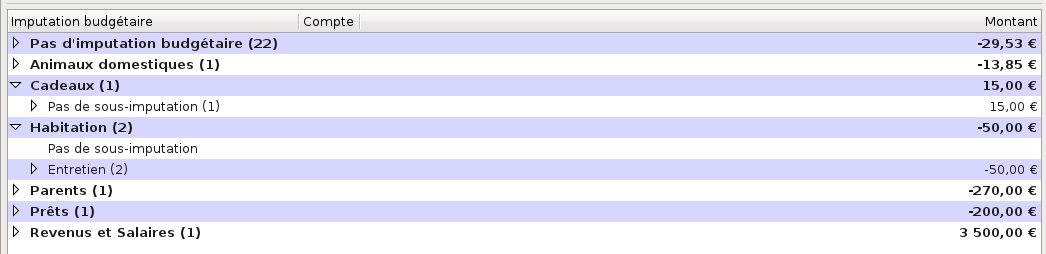
\includegraphics[scale=0.5]{image/screenshot/budgetarylines_list}
\end{center}
\caption{Liste des imputations et des sous-imputations budgétaires}
\label{budgetarylines-list-img}
\end{figure}
% image centrée
\fi

Elle affiche en haut la barre des libellés des colonnes ; ses champs d'affichage sont les suivants :
\begin{itemize}
	 \item le nom de l'imputation ou de la sous-imputation budgétaire ;
	 \item le compte concerné ;
	 \item le montant total des opérations affectées aux imputations et sous-imputations budgétaires, et le montant de chaque opération affectée à ces imputations et sous-imputations budgétaires si leurs lignes sont déroulées.
\end{itemize}

Vous pouvez déplacer la liste des imputations budgétaires vers le haut ou vers le bas avec la molette de la souris, ou bien avec la souris et l'ascenseur vertical. Le déplacement éventuel vers la gauche ou la droite se fait avec la souris et l'ascenseur horizontal.

Pour  afficher les sous-imputations d'une imputation budgétaire, cliquez sur le petit triangle à gauche de son nom, ou bien double-cliquez sur sa ligne ;
% ou bien sélectionnez-la et appuyez sur la barre d'espace (non fonctionnel) 
 cela affiche le libellé  de toutes les sous-imputations, et éventuellement, en première position, \indexword{\menu{Pas de sous-imputation}}\index{sous-imputations budgétaires !pas de sous-imputation}.
 
\textbf{Note} : ces triangles peuvent être remplacés, en fonction du thème de l'environnement de bureau ou du gestionnaire de fenêtres que vous utilisez, par d'autres caractères tels que +, -, >, <, etc. 

%le seul moyen de dérouler la liste est de cliquer sur le petit triangle. il devrait y avoir un moyen avec le clavier, comme ça existe avec le formulaire de saisie, où l'on peut utiliser la barre d'espace pour le moyen de paiement, ou la touche flèche bas pour la catégorie...

% espace pour changement de thème
\vspacepdf{5mm}
Vous pouvez afficher plusieurs \indexword{imputations budgétaires déroulées}\index{imputations budgétaires !déroulées}. Pour ne plus les afficher, \indexword{enroulez les imputations budgétaires}\index{imputations budgétaires !enroulées} en cliquant sur le petit triangle à gauche de leur nom, ou bien double-cliquez sur leur ligne. Vous pouvez aussi dérouler ou enrouler toutes les imputations budgétaires de la liste, en cliquant sur l'outil \menu{Affichage}\index{affichage !imputations budgétaires} dans la barre d'outils et en choisissant \menu{Vue des imputations et des sous-imputations}. Pour afficher seulement les imputations, cliquez sur l'outil \menu{Affichage} dans la barre d'outils et choisissez \menu{Vue des imputations uniquement}.

Les imputations et sous-imputations de votre fichier de comptes sont affichées par ordre alphabétique, avec deux exceptions : la première imputation affichée est toujours l'imputation de libellé \indexword{\menu{Pas d'imputation}}\index{imputations budgétaires !pas d'imputation}, qui reçoit toutes les opérations dont l'imputation n'est pas définie, et, à l'intérieur d'une imputation, la première sous-imputation affichée est toujours la sous-imputation de libellé \indexword{\menu{Pas de sous-imputation}} \index{sous-imputations budgétaires !pas de sous-imputation}, qui reçoit toutes les opérations dont la sous-imputation n'est pas définie.

Le nombre d'opérations affectées à chaque imputation ou sous-imputation budgétaire s'affiche, entre parenthèses, à la suite de son nom, et le montant total des opérations affectées à ces imputations ou sous-imputations budgétaires s'affiche dans la colonne \menu{Montant}, à droite sur la même ligne. 

% Bogue connu  : en cliquant sur une ligne de catégories, la barre d'information devrait afficher le total, mais n'affiche que 0.

\ifIllustration
\else
% espace avant Attention ou Note  : 5 mm
\vspacepdf{5mm}
\fi

\textbf{Note} : vous pouvez configurer la \indexword{devise des totaux}\index{devise !totaux} de toutes les (sous-) imputations budgétaires dans le menu \menu{Édition - Préférences} (voir la section \vref{setup-display-third-currencies}, \menu{Devises des totaux}).


\section{Sélection d'une (sous-) imputation budgétaire\label{budgetarylines-selection}}


Pour sélectionner une imputation ou une sous-imputation budgétaire, vous avez deux moyens :

\begin{itemize}
	 \item cliquez sur sa ligne ;
	 \item déplacez la sélection avec les touches du clavier \key{Flèche Haut}, \key{Flèche Bas}, \key{Page Haut} ou \key{Page Bas}.
\end{itemize}

Le nom de l'imputation ou sous-imputation budgétaire apparaît alors sur fond rose{\couleur}.

% espace pour changement de thème
\vspacepdf{5mm}
Un menu contextuel est disponible par un clic-droit sur la liste des imputations budgétaires ; selon la ligne sélectionnée, vous pouvez exécuter les fonctions suivantes :

\begin{itemize}
	 \item pour une imputation budgétaire : \menu{Éditer l'imputation sélectionnée} ;
	 \item pour l'imputation budgétaire \menu{Pas de sous-imputation} :
		\begin{itemize}
			 \item si elle est vide :\menu{Éditer l'imputation sélectionnée},
			 \item si elle contient des opérations : \menu{Transférer les opérations dans une autre sous-imputation},
		\end{itemize}
	 \item pour	une sous-imputation quelconque :	
		\begin{itemize}
			 \item \menu{Éditer la sous-imputation sélectionnée},
			 \item \menu{Gérer les sous-imputations},			 
		\end{itemize}		
	 \item pour une opération quelconque : \menu{Transférer des opérations identiques dans une autre sous-imputation}.	
\end{itemize}


\section{Les opérations d'une (sous-) imputation budgétaire\label{budgetarylines-transactions}}


Une ligne de libellé \menu{Pas de sous-imputation} se comporte exactement comme une ligne de sous-imputation budgétaire.

Pour afficher les opérations, cliquez sur le petit triangle à gauche du libellé  \menu{Pas de sous-imputation} ou celui d'une sous-imputation, ou bien double-cliquez sur sa ligne,
% ou bien sélectionnez-la et appuyez sur la barre d'espace (non fonctionnel),
 ce qui déroule la liste. Les opérations sont alors décrites sur une seule ligne, avec leur date, leur remarque éventuelle, le nom du compte concerné et leur montant.

\textbf{Note} : ces triangles peuvent être remplacés, en fonction du thème de l'environnement de bureau ou du gestionnaire de fenêtres que vous utilisez, par d'autres caractères tels que +, -, >, <, etc. 

%le seul moyen de dérouler la liste est de cliquer sur le petit triangle. il devrait y avoir un moyen avec le clavier, comme ça existe avec le formulaire de saisie, où l'on peut utiliser la barre d'espace pour le moyen de paiement, ou la touche flèche bas pour la catégorie...

% espace pour changement de thème
\vspacepdf{5mm}
Vous pouvez afficher plusieurs lignes de \indexword{sous-imputations budgétaires déroulées}\index{sous-imputations budgétaires !déroulées}. Pour ne plus les afficher, \indexword{enroulez les  opérations}\index{sous-imputations budgétaires !enroulées} d'une sous-imputation budgétaire en cliquant sur le petit triangle à gauche de son nom, ou bien double-cliquez sur leur ligne. Vous pouvez aussi dérouler ou enrouler toutes les opérations de toutes les imputations et sous-imputations budgétaires de la liste, en cliquant sur l'outil \menu{Affichage}\index{affichage !sous-imputations} dans la barre d'outils, et en faisant votre choix entre \menu{Vue des imputations uniquement}, \menu{Vue des imputations et sous-imputations} ou \menu{Vue complète}.

%espace pour changement de thème
\vspacepdf{5mm}
Vous pouvez \indexword{déplacer une opération}\index{sous-imputations budgétaires !déplacement d'opération} d'une sous-imputation vers une autre sous-imputation de la liste en sélectionnant cette opération et en faisant un glisser-déplacer sur la sous-imputation cible, exactement à l'endroit où son nom est entouré d'une bordure pointillée.

%espace pour changement de thème
\vspacepdf{5mm}
Un \indexword{double-clic} sur une ligne d'opération d'une imputation\index{imputations budgétaires !double-clic sur opération} ou d'une sous-imputation budgétaire\index{sous-imputations budgétaires !double-clic sur opération} ferme l'onglet \menu{Imputations budgétaires}, ouvre l'onglet \menu{Comptes} et le sous-onglet du compte contenant cette opération, sélectionne l'opération concernée et l'affiche dans le formulaire de saisie. De cette façon, cette opération peut être affichée et modifiée facilement.


\section{Création d'une (sous-) imputation budgétaire\label{budgetarylines-new}}


La création d'une imputation budgétaire au cours de la saisie d'une opération n'est possible que si le champ d'information a été créé préalablement dans le formulaire de saisie des opérations (voir la section \vref{setup-form}, \menu{Formulaire des opérations}).

\ifIllustration
% image entourée par un paragraphe ( picins)
% Pas de référence à l'illustration car erreur de numéro de figure avec picins.
% supprimé car en html les figures entourées ne sont pas numérotées, et la numérotation des figures centrées décalée par rapport au pdf
%\piccaption{Création d'une imputation budgétaire}
\label{budgetarylines-new-img}
\parpic[r]{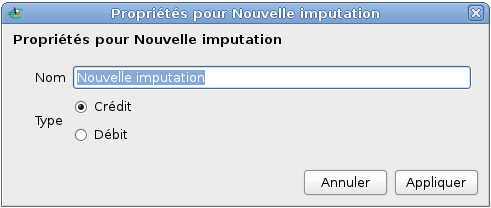
\includegraphics[scale=0.5]{image/screenshot/budgetarylines_new}}
% image entourée par un paragraphe ( picins)
\fi

\noindent La façon la plus immédiate pour créer une imputation ou une sous-imputation budgétaire est de saisir son nom au cours de la création d'une nouvelle opération dans l'onglet des comptes (voir la section \vref{transactions-fillcombo}, \menu{Nouveau tiers, catégorie ou imputation budgétaire}) ; mais vous pouvez aussi en créer ici, en cliquant sur l'outil \menu{Nouvelle imputation} ou \menu{Nouvelle sous-imputation}. Une boîte de dialogue s'ouvre ; suivant le cas, renseignez le nom de l'imputation et cochez si elle contiendra des crédits ou des débits, ou renseignez uniquement le nom de la sous-imputation, puis validez.

% espace pour changement de thème
\vspacepdf{5mm}
L'outil \menu{Nouvelle sous-imputation}\label{budgetarylines-newsub} de la barre d'outils ne devient actif que lorsqu'une imputation budgétaire est sélectionnée dans la liste.

\ifIllustration
% espace après image entourée
\vspacehevea{5mm}
\fi


\section{Modification d'une (sous-) imputation budgétaire\label{budgetarylines-modify}}


Pour modifier une imputation ou une sous-imputation budgétaire, procédez comme suit :
% espace avant image 5mm
\vspacepdf{3mm}

\begin{enumerate}
	\ifIllustration
	% image entourée par un paragraphe ( picins)
	% Pas de référence à l'illustration car erreur de numéro de figure avec picins.
	\pichskip{10mm}
	% supprimé car en html les figures entourées ne sont pas numérotées, et la numérotation des figures centrées décalée par rapport au pdf
	%\piccaption{Modification d'une imputation budgétaire}
	\label{budgetarylines-infos-img}
	\parpic[r]{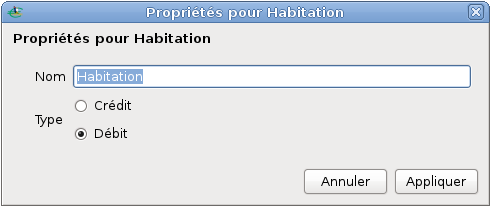
\includegraphics[scale=0.51]{image/screenshot/budgetarylines_infos}}
	% image entourée par un paragraphe ( picins)
	\fi
	 \item sélectionnez sa ligne ;
	 \item cliquez sur l'outil \menu{Éditer} dans la barre d'outils, ou sélectionnez \menu{Éditer l'imputation sélectionnée} ou \menu{Éditer la sous-imputation sélectionnée} dans le menu contextuel accessible par un  clic-droit ;
	 \item une boîte de dialogue s'ouvre : modifiez son nom et, uniquement pour les imputations, son type (crédit ou débit) ;
	 \item validez.
\end{enumerate}

\ifIllustration
% espace après inage entourée
\vspacehevea{6mm}
\fi

\section{Transfert d'opérations dans une autre sous-imputation\label{budgetarylines-transfer}}


Vous pouvez \indexword{transférer des opérations dans une autre sous-imputation}\index{sous-imputations budgétaires !transfert d'opérations} ayant pour point commun soit le tiers, soit la remarque, soit les deux ; pour cela, procédez comme suit :
% espace avant image 5mm
\vspacepdf{3mm}

% Pas de référence à l'illustration car erreur de numéro de figure avec picins.
\begin{enumerate}
	% image entourée par un paragraphe ( picins)
	\ifIllustration
	\pichskip{10mm}
	% supprimé car en html les figures entourées ne sont pas numérotées, et la numérotation des figures centrées décalée par rapport au pdf
	%\piccaption{Transfert d'opérations identiques dans une autre sous-imputation}
	\label{budgetarylines_transfer-img}
	\parpic[r]{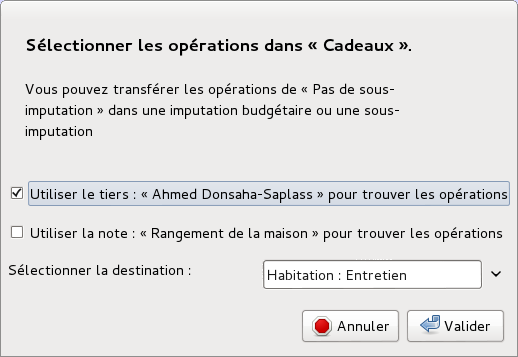
\includegraphics[scale=0.51]{image/screenshot/budgetarylines_transfer}}
	\fi
	% image entourée par un paragraphe ( picins)
	 \item sélectionnez la ligne de l'opération concernée ;
	 \item sélectionnez \menu{Transférer des opérations identiques dans une autre sous-imputa\dash tion}, dans le menu contextuel accessible par un  clic-droit ;
	 \item une boîte de dialogue s'affiche ; cochez l'une des deux cases \menu{Utiliser le tiers\ldots{ }} et \menu{Utiliser la note\ldots{ }} ou les deux selon votre besoin ;
	 \item renseignez le champ libellé \menu{Sélectionner la destination}, ou choisissez une imputation et une sous-imputation dans la liste déroulante ;
	 \item validez.
\end{enumerate}

\textbf{Note} : la saisie du champ libellé \menu{Sélectionner la destination} bénéficie de la fonction d'\indexword{auto-complètement}\index{champ de saisie !auto-complètement}.

\ifIllustration
% espace après image entourée
\vspacehevea{18mm}
\fi


\section{Gestion des sous-imputations budgétaires\label{budgetarylines-management}}


Vous pouvez modifier l'organisation de vos sous-imputations budgétaires en \indexword{déplaçant le contenu d'une sous-imputation}\index{sous-imputations budgétaires !déplacement d'opération} vers une autre ou vers une nouvelle imputation. Pour cela, sélectionnez une sous-imputation, puis cliquez-droit et choisissez dans le menu contextuel : 


\begin{itemize}
	 \item pour la sous-imputation \menu{Pas de sous-imputation} : sélectionnez \menu{Transférer les opérations dans une autre sous-imputation} : une fenêtre s'affiche ; sélectionnez la destination dans la liste déroulante, puis validez ;

	 \item pour les autres sous-imputations : sélectionnez \menu{Gérer les sous-imputations}, une fenêtre s'affiche ; sélectionnez l'action désirée \ifIllustration \refimage{budgetarylines-management-img} :
	 \else  :
	 \fi
		\begin{itemize}
			 \item \menu{Transférer les opérations dans une imputation ou une sous-imputation} : sélectionnez l'imputation de destination dans la liste déroulante, puis validez,
			 \item \menu{Transférer \og nom de la sous-imputation sélectionnée \fg{} dans une autre imputation} : sélectionnez l'imputation de destination dans la liste déroulante, puis validez,
			 \item \menu{Convertir \og nom de la sous-imputation sélectionnée \fg{} en nouvelle imputation} : validez, la sous-imputation est devenue une imputation.
		\end{itemize}
\end{itemize}

\ifIllustration
% image centrée
\begin{figure}[hbp]
\begin{center}
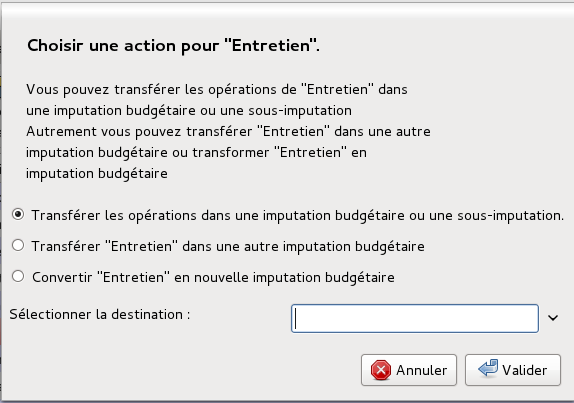
\includegraphics[scale=0.48]{image/screenshot/budgetarylines_management}
\end{center}
\caption{Gestion des sous-imputations budgétaires}
\label{budgetarylines-management-img}
\end{figure}
% image centrée
\fi


\section{Suppression d'une (sous-) imputation budgétaire\label{budgetarylines-delete}}


Pour supprimer une imputation ou une sous-imputation budgétaire, procédez comme suit :
% espace avant image 5mm
\vspacepdf{3mm}

\begin{enumerate}
	\ifIllustration
	% image entourée par une liste (picins)
	% Pas de référence à l'illustration car erreur de numéro de figure avec picins.
	\pichskip{11mm}
	% supprimé car en html les figures entourées ne sont pas numérotées, et la numérotation des figures centrées décalée par rapport au pdf
	%\piccaption{Suppression d'une sous-imputation budgétaire}
	\label{budgetarylines-delete-img}
	\parpic[r]{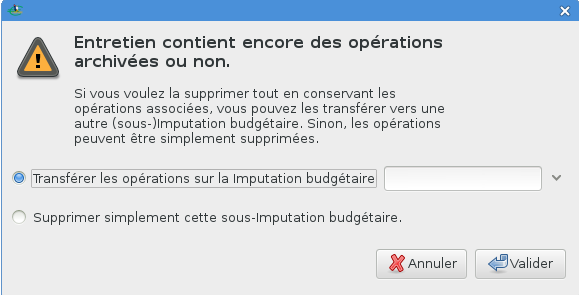
\includegraphics[scale=0.5]{image/screenshot/budgetarylines_delete}}
	% image entourée par une liste (picins)
	\fi
	
	 \item sélectionnez-la dans la liste ;
	 \item cliquez sur l'outil \menu{Supprimer} dans la barre d'outils ;
	 \item une  boîte de dialogue s'ouvre et vous propose soit de ré-affecter les opérations de cette (sous-) imputation vers une autre (sous-) imputation budgétaire, soit de la supprimer purement et simplement, y compris toutes ses opérations ; 
	 \item faites votre choix puis validez.
\end{enumerate}

\strong{Attention} : la suppression d'une imputation ou d'une sous-imputation budgétaire est \indexword{irréversible}\index{opération !irréversible} ! 

% espace avant Attention ou Note  : 5 mm
\vspacepdf{5mm}
\textbf{Note} : si la (sous-) imputation budgétaire que vous voulez supprimer ne contient aucune opération, aucune boîte de dialogue ne s'ouvrira et Grisbi la supprimera immédiatement.

\ifIllustration
% espace après inage entourée
\vspacehevea{3mm}
\fi


\section{Import et export\label{budgetarylines-importexport}}


Grisbi vous permet d'importer ou d'exporter les imputations budgétaires d'un fichier de comptes, ce qui peut éviter de recréer tout un ensemble d'imputations budgétaires si on peut le trouver ailleurs déjà fait.


\subsection{Import d'une liste de (sous-) imputations budgétaires\label{budgetarylines-importexport-import} }

Pour \indexword{importer une liste de (sous-) imputations budgétaires}\index{imputations budgétaires !import}\index{sous-imputations budgétaires !import}, procédez comme suit :

\begin{enumerate}
	 \item cliquez sur l'outil \menu{Importer} dans la barre d'outils : une fenêtre de gestionnaire de fichiers s'affiche ;
	 \item choisissez le répertoire et le nom du fichier à importer, dont l'\indexword{extension} doit être \file{.igsb}\index{extension !.igsb} ;
	 \item cliquez sur le bouton \menu{Ouvrir} ; 
	 \item une boîte de dialogue vous informe, éventuellement, que ce fichier contient déjà des opérations, et que sa liste d'imputations budgétaires et celle de votre fichier de comptes en cours seront fusionnées. Si cela vous convient, validez par le bouton \menu{Valider}.
\end{enumerate}

% espace avant Attention ou Note  : 5 mm
\vspacepdf{5mm}
\strong{Attention} : d'une manière générale, il est déconseillé d'avoir des accents ou des espaces dans les noms des répertoires et fichiers utilisés par Grisbi. Si c'est le cas, renommez-les maintenant. Par exemple, les espaces peuvent être remplacées par des tirets bas (\_). 
% espace après Attention ou Note  : 5 mm
\vspacepdf{5mm}

Si vous avez validé, il vous appartient ensuite de supprimer une à une toutes les imputations budgétaires que vous ne voulez pas garder, ou d'en créer de nouvelles.

Si vous commencez un fichier de comptes neuf, vous aurez avantage à supprimer les imputations budgétaires existantes par défaut avant d'importer une autre liste.


\subsection{Import d'une liste de (sous-) catégories\label{budgetarylines-importexport-importCategories} }

Si vous voulez vous servir de votre liste de (sous-) catégories comme base pour établir votre liste d'imputations budgétaires, vous devez d'abord exporter votre liste de (sous-) catégories dans un fichier. Pour cela, reportez-vous à la section \vref{categories-importexport-export}, \menu{Export de vos (sous-) catégories}. 

Puis, pour \indexword{importer votre liste de (sous-) catégories}\index{catégories !import}\index{sous-catégories !import}, procédez comme suit : 

\begin{enumerate}
	 \item cliquez sur l'outil \menu{Importer} dans la barre d'outils : une fenêtre de gestionnaire de fichiers s'affiche ;
	 \item dans le coin en bas et à droite de la fenêtre, sélectionnez dans la liste déroulante \menu{Fichier des catégories Grisbi (*.cgsb}) ;
	 \item choisissez le répertoire et le nom du fichier à importer, dont l'\indexword{extension} doit être \file{.cgsb}\index{extension !.cgsb} ;
	 \item cliquez sur le bouton \menu{Ouvrir} ; 
	 \item une boîte de dialogue vous propose, soit de fusionner votre liste de catégories avec votre liste d'imputations budgétaires existantes, soit que votre liste de catégories remplace votre liste d'imputations budgétaires existantes ; dans le cas de la fusion, cliquez sur le bouton \menu{Valider}, sinon dans le cas du remplacement, cliquez sur le bouton \menu{Remplacer l'existant}.
\end{enumerate}


\subsection{Export de vos (sous-) imputations budgétaires\label{budgetarylines-importexport-budgetary}}

Pour \indexword{exporter la liste de vos (sous-) imputations budgétaires}\index{imputations budgétaires !export}\index{sous-imputations budgétaires !export}, procédez comme suit :

\begin{enumerate}
	 \item cliquez sur l'outil \menu{Exporter} dans la barre d'outils : une fenêtre de gestionnaire de fichiers s'affiche ;
	 \item saisissez le nom du fichier à exporter, dont l'\indexword{extension} sera \file{.igsb}\index{extension !.igsb} :
	 \item choisissez son répertoire de destination :
	 \item cliquez sur le bouton \menu{Enregistrer}.
\end{enumerate}

% espace avant Attention ou Note  : 5 mm
\vspacepdf{5mm}
\strong{Attention} : d'une manière générale, il est déconseillé d'avoir des accents ou des espaces dans les noms des répertoires et fichiers utilisés par Grisbi. Si c'est le cas, renommez-les maintenant. Par exemple, les espaces peuvent être remplacées par des tirets bas (\_). 


%\subsection{Format des fichiers d'imputations budgétaires}
%
%Ces fichiers sont enregistrés au format \file{XML}, comme le fichier de comptes.
%La structure du fichier est identique à celle du fichier de comptes, section
%\file{Imputations budgétaires} (voir l'annexe \vref{xml-budgetarylines})